\documentclass{ximera}  
\title{Bisection Method}  
\begin{document}  
\begin{abstract}  
We give an introduction to finding roots using the Bisection Method.
\end{abstract}  
\maketitle

\section{The Intermediate Value Theorem}

The Intermediate Value Theorem (IVT) simply states that if $f(x)$ is a continuous function on the interval $[a,b]$, then it takes on any given value between $f(a)$ and $f(b)$. In other words, if $f(x)$ is a continuous function, then any horizontal line between $f(a)$ and $f(b)$ intersects the graph of $f(x)$. Note that this theorem does not give the number or location of such intersections. The Desmos interactive graph below gives an example of the IVT in action.

\desmos{uroxd0wmuh}{800}{600}

We will use the IVT to come up with numerical approximations to solutions of equations of the form $f(x)=0$. 

\section{The Bisection Method}

The Bisection Method makes use of the IVT in a special situation: when $f(a)$ and $f(b)$ are nonzero values of opposite sign.

Suppose you are given a function $f(x)$ and you are interested in finding at least one solution to the equation $f(x)=0$. Furthermore, suppose that $f(0)=2$, $f(4)=-3$, and $f(x)$ is continuous on the interval $[0,4]$. Then, by the IVT, we know that our equation has at least one solution in the interval $[0,4]$. We can narrow down our search by computing $f(2)$ (here $2$ is the midpoint of the interval). If $f(2)=0$, then we found a solution! If $f(2)>0$, then by the IVT, there is a solution in the interval $[2,4]$. Otherwise, if $f(2)<0$, then by the IVT, there is a solution in the inteval $[0,2]$. We can repeat this procedure until we get an approximation that is ``close enough" to a solution. At each step, we trim down the length of the inteval containing a solution in half, bounding the size of our possible error to half the size of the remaining interval. 

It is possible that we may never find the exact value of a solution or that we may miss some solutions. Try, for example, to use the procedure above to find solutions to $x^3-2x=0$ on the interval $[-5,5]$.

We can summarize the Binomial Method using the following flowchart. Here we assume that $a<b$, $f(x)$ is continuous on $[a,b]$ and $error>0$.

\begin{center}
	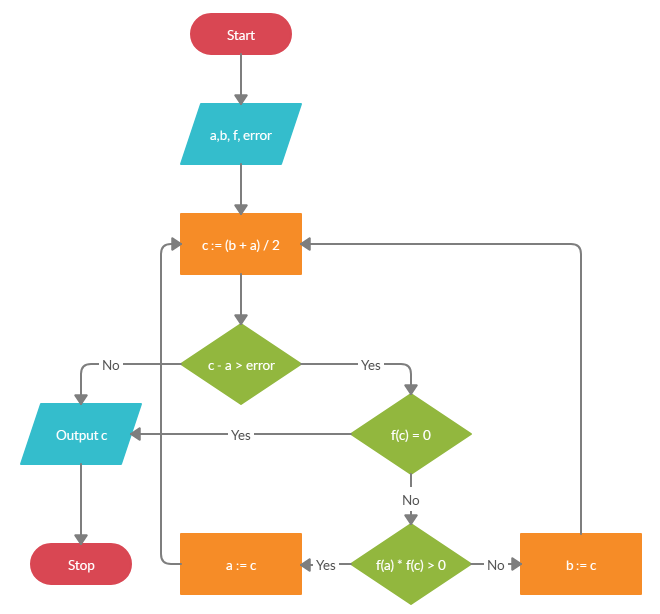
\includegraphics{bisection.png}
\end{center}

Converting this to code gives the following:

\begin{verbatim}
==============================
def bisection(a,b,f,error):
        c = (b+a)/2
        while c-a > error:
                if f(c) == 0:
                        return c
                elif f(a)*f(c) > 0:
                        a = c
                else:
                        b = c
                c = (b+a)/2
        return c
==============================
\end{verbatim}

Note that we use the fact that $x\cdot y>0$ implies that both $x$ and $y$ have the same sign.

The Binomial Method has several advantages and one major dissadvantage. It is an algorithm that is relatively easy to code, requires very few assumptions on the function, and always converges to some solution. The biggest dissadvantag of this method is that the convergence to a solution may be very slow compared to other methods (to be seen in the next section).

Note that we can also use the Bisection Method to solve equations of the form $f(x)=k$ by solving $g(x)=0$ with $g(x)=f(x)-k$.

\section{Problems}

Note that for the questions below, the hint contains the solution.

\begin{question}
\end{question}

\section{Workspace}

\begin{sageCell}
# Use this cell to solve the above questions.
\end{sageCell}

\end{document}
